%!TEX root = ../my_thesis.tex
\chapter{Results}


\section{Calcite experiment}

In this experiment we've observed the dissolution of calcite ($CaCO_3$) with water. We have decided to choose this reaction because the chemical reaction leading to the dissolution is simple. Moreover, it is abundant and geologically important material.\cite{hillner1992atomic} Indeed, a better understanding of calcite dissolution (mass transfer across the surface) is important for the improvement of models of contaminant transport and global warming. \cite{liang1996dissolution}

In this experiment, we should observe \cite{Hillner19921387}
\begin{equation}\label{calcite}
CaCO_3(calcite) + H_20 \rightarrow Ca^{2+} + HCO_3^- + OH^- 
\end{equation}

We have used our double PID feedback system and /InsertTipType. Calcite dissolution is an interesting process to observe with a high speed AFM. The whole process lasts X min which is observable with our setup. With a commercial AFM, that takes a few minutes for a raster scan, the dissolution process is hard to monitor (only a few pictures).

We have mounted our calcite sample on top of the fast piezo-electrical ceramics. Also, we have stuck a plastic cover underneath the piezo for the water. THe calcite will dissolve itself with a losange pattern. It is linked to its original geometry.

We have imaged the same sample with different parameters: scan size, number of spirals and scanning time.

\begin{figure}[H]
  \centering
  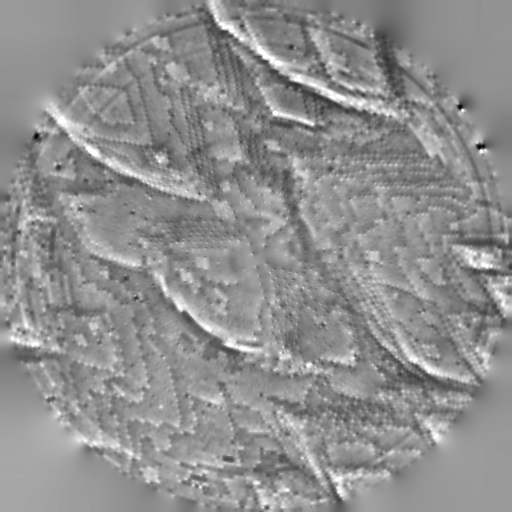
\includegraphics[scale=0.5]{images/006_X10s50l10m_MOv2_17.png}
    \caption{Calcite dissolution}
  \label{Calcite dissolution}
\end{figure}

